\documentclass[10pt]{beamer}
\usepackage[english]{babel}
\usepackage[utf8]{inputenc}
\usepackage[T1]{fontenc}
\usepackage{helvet}

%-------------------------------------------------------
% INFORMATION IN THE TITLE PAGE
%-------------------------------------------------------

\newcommand{\cstitle}{\textbf{Bioinformática - Introducción}}
\subtitle[]{CPO}
\newcommand{\cscourseCode}{Matemáticas discretas II}
\newcommand{\csauthor}{PhD(c). Vicente Machaca Arceda}
\institute[UNSA]{Universidad de Ingeniería y Tecnología}
\newcommand{\csemail}{vmachaca@utec.edu.pe}
\newcommand{\instituteabr}{UTEC}
\newcommand{\nameUp}{}
\date{2022-I}
\title[\cscourseCode]{\cstitle}
\author{\csauthor}
%%%%%%%%%%%%%%%%%

%-------------------------------------------------------
% CHOOSE THE THEME
%-------------------------------------------------------
\def\mycmd{0} % UNSA
\def\mycmd{1} % SALLE
\def\mycmd{2} % UTEC
%-------------------------------------------------------

\if\mycmd0
\usepackage{csformat}
\newcommand{\chref}[3][blue]{\href{#2}{\color{#1}{#3}}}%

\fi

\if\mycmd1
\usetheme[]{Feather}
\newcommand{\chref}[2]{	\href{#1}{{\usebeamercolor[bg]{Feather}#2}} }
\fi

\if\mycmd2
\usetheme{UTEC2020}	
\newcommand{\chref}[3][blue]{\href{#2}{\color{#1}{#3}}}%
\fi

\newcommand{\1}{
        	\setbeamertemplate{background}{
        		
\includegraphics[width=\paperwidth,height=\paperheight]{img/1}
        		\tikz[overlay] \fill[fill opacity=0.75,fill=white] (0,0) rectangle (-\paperwidth,\paperheight);
        	}
}



%-------------------------------------------------------
% THE BODY OF THE PRESENTATION
%-------------------------------------------------------

\begin{document}


\AtBeginSubsection[]
{
    \begin{frame}
        \frametitle{Contenido}
        \tableofcontents[currentsubsection]
    \end{frame}
}


%-------------------------------------------------------
% THE TITLEPAGE
%-------------------------------------------------------

\if\mycmd0
\maketitle
\fi

\if\mycmd1 % MY THEME
\1{
	\begin{frame}[plain,noframenumbering] 
		\titlepage 
\end{frame}}
\fi

\if\mycmd2
\begin{frame}
	\titlepage
\end{frame}
\fi
%-------------------------------------------------------
%-------------------------------------------------------

\begin{frame}{Contenido}
	\tableofcontents
\end{frame}

%-------------------------------------------------------
%-------------------------------------------------------

% fuente: http://mate.cucei.udg.mx/matdis/1rel/1rel4.htm

\section{Introducción}

%%%%%%%%%%%%%%%%%%%%%%%%%%%%%%%%%%%%%%%%%%%%%%%%%%%%%%%%
%\subsection{Objectives}
%%%%%%%%%%%%%%%%%%%%%%%%%%%%%%%%%%%%%%%%%%%%%%%%%%%%%%%%

%-------------------------------------------------------
%-------------------------------------------------------
%\begin{frame}{Objectives}{}
%	\begin{itemize}
	%		\item<1-> Understand what is Bioinformatics. 
	%		\item<2-> Learn areas of research of Bioinformatics related to COVID-19.
	%	\end{itemize}
%\end{frame}
%-------------------------------------------------------
%-------------------------------------------------------


%%%%%%%%%%%%%%%%%%%%%%%%%%%%%%%%%%%%%%%%%%%%%%%%%%%%%%%%
\subsection{Presentación}
%%%%%%%%%%%%%%%%%%%%%%%%%%%%%%%%%%%%%%%%%%%%%%%%%%%%%%%%

%-------------------------------------------------------
%-------------------------------------------------------
\begin{frame}{Presentación}{}
	\begin{itemize}
		\item<1-> PhD(c). Vicente Enrique Machaca Arceda. 
		\item<2-> Profesor UTEC (TP).
		\item<3-> Investigador en Bioinformática y Aprendizaje de Maquina.	
		\item<4-> \chref{https://scholar.google.com/citations?user=Y2taS2MAAAAJ&hl=es&oi=ao}{Index-h 5}.  	
	\end{itemize}
\end{frame}
%-------------------------------------------------------
%-------------------------------------------------------

%-------------------------------------------------------
%-------------------------------------------------------
\begin{frame}{Presentación}{Publicaciones}
	\begin{table}[]
		\setlength{\tabcolsep}{0.5em} % for the horizontal padding
		{\renewcommand{\arraystretch}{1.4}% for the vertical padding
			\begin{tabular}{llp{7cm}}
				\textbf{Year} & \textbf{Country} & \textbf{Title}                                                                                                              \\
				\hline
				2020          & USA              & Small Ship Detection on Optical Satellite Imagery with YOLO and YOLT                                                        \\
				2018          & Brasil           & Fast Car Crash Detection in Video                                                                                           \\
				2016          & Chile            & Fast Face Detection in Violent Video Scenes                                                                                 \\
				2016          & Costa Rica       & Real Time Violence Detection in Video with ViF and Horn-Schunck                                                             \\
				2016          & Costa Rica       & Optimization model for face detection in video sequences                                                                    \\
				2015          & Chile            & Real Time Violence Detection in Video                                                                                      
			\end{tabular}
		}
	\end{table}
\end{frame}
%-------------------------------------------------------
%-------------------------------------------------------

%-------------------------------------------------------
%-------------------------------------------------------
\begin{frame}{Presentation}{Publications}
	\begin{table}[]
		\setlength{\tabcolsep}{0.5em} % for the horizontal padding
		{\renewcommand{\arraystretch}{1.4}% for the vertical padding
			\begin{tabular}{llp{7cm}}
				\textbf{Year} & \textbf{Country} & \textbf{Title}                                                                                                              \\
				\hline
				2022          &  USA                & ArgosMol: A Web Tool for Protein Structure Prediction and Visualization             \\
				2021          &  Chapter                & COVID-19 Pandemic: Analysis and Statistics of Confirmed Cases             \\
				2020          &  Canada          & An Analysis of k-Mer Frequency Features with Machine Learning Models for Viral Subtyping of Polyomavirus and HIV-1 Genomes                                                        \\
				
				2020          & Canada           & An analysis of k-mer frequency features with SVM and CNN for viral subtyping classification \\
				2020          & Canada           & Forecasting time series with Multiplicative Trend Exponential Smoothing and LSTM: COVID-19 case study                       \\
				
				
			\end{tabular}
		}
	\end{table}
\end{frame}
%-------------------------------------------------------
%-------------------------------------------------------

%%%%%%%%%%%%%%%%%%%%%%%%%%%%%%%%%%%%%%%%%%%%%%%%%%%%%%%%
\subsection{Objetivos}
%%%%%%%%%%%%%%%%%%%%%%%%%%%%%%%%%%%%%%%%%%%%%%%%%%%%%%%%

%-------------------------------------------------------
%-------------------------------------------------------
\begin{frame}{Objetivos}{}
	\begin{block}{}
		\begin{itemize}
			\item Conocer que es la Bioinformática y como se relaciona con las Ciencias de la Computación.
			\item Conocer las principales aplicaciones de la Bioinformática.
		\end{itemize}
	\end{block}
\end{frame}
%-------------------------------------------------------
%-------------------------------------------------------

%%%%%%%%%%%%%%%%%%%%%%%%%%%%%%%%%%%%%%%%%%%%%%%%%%%%%%%%
\subsection{Motivación}
%%%%%%%%%%%%%%%%%%%%%%%%%%%%%%%%%%%%%%%%%%%%%%%%%%%%%%%%

%-------------------------------------------------------
%-------------------------------------------------------
\begin{frame}{Muertes por COVID-19}{}
	\begin{columns}
		\begin{column}{0.48\textwidth}
			\begin{block}{}
				\textbf{213 mil} muertes por COVID en Perú \cite{worldometrcovid2022}.
			\end{block}
			\begin{block}{}
				\textbf{6.29 millones} de muertes por COVID en el mundo \cite{worldometrcovid2022}.
			\end{block}
		\end{column}
		\begin{column}{0.48\textwidth}
			\begin{figure}[]
				\centering
				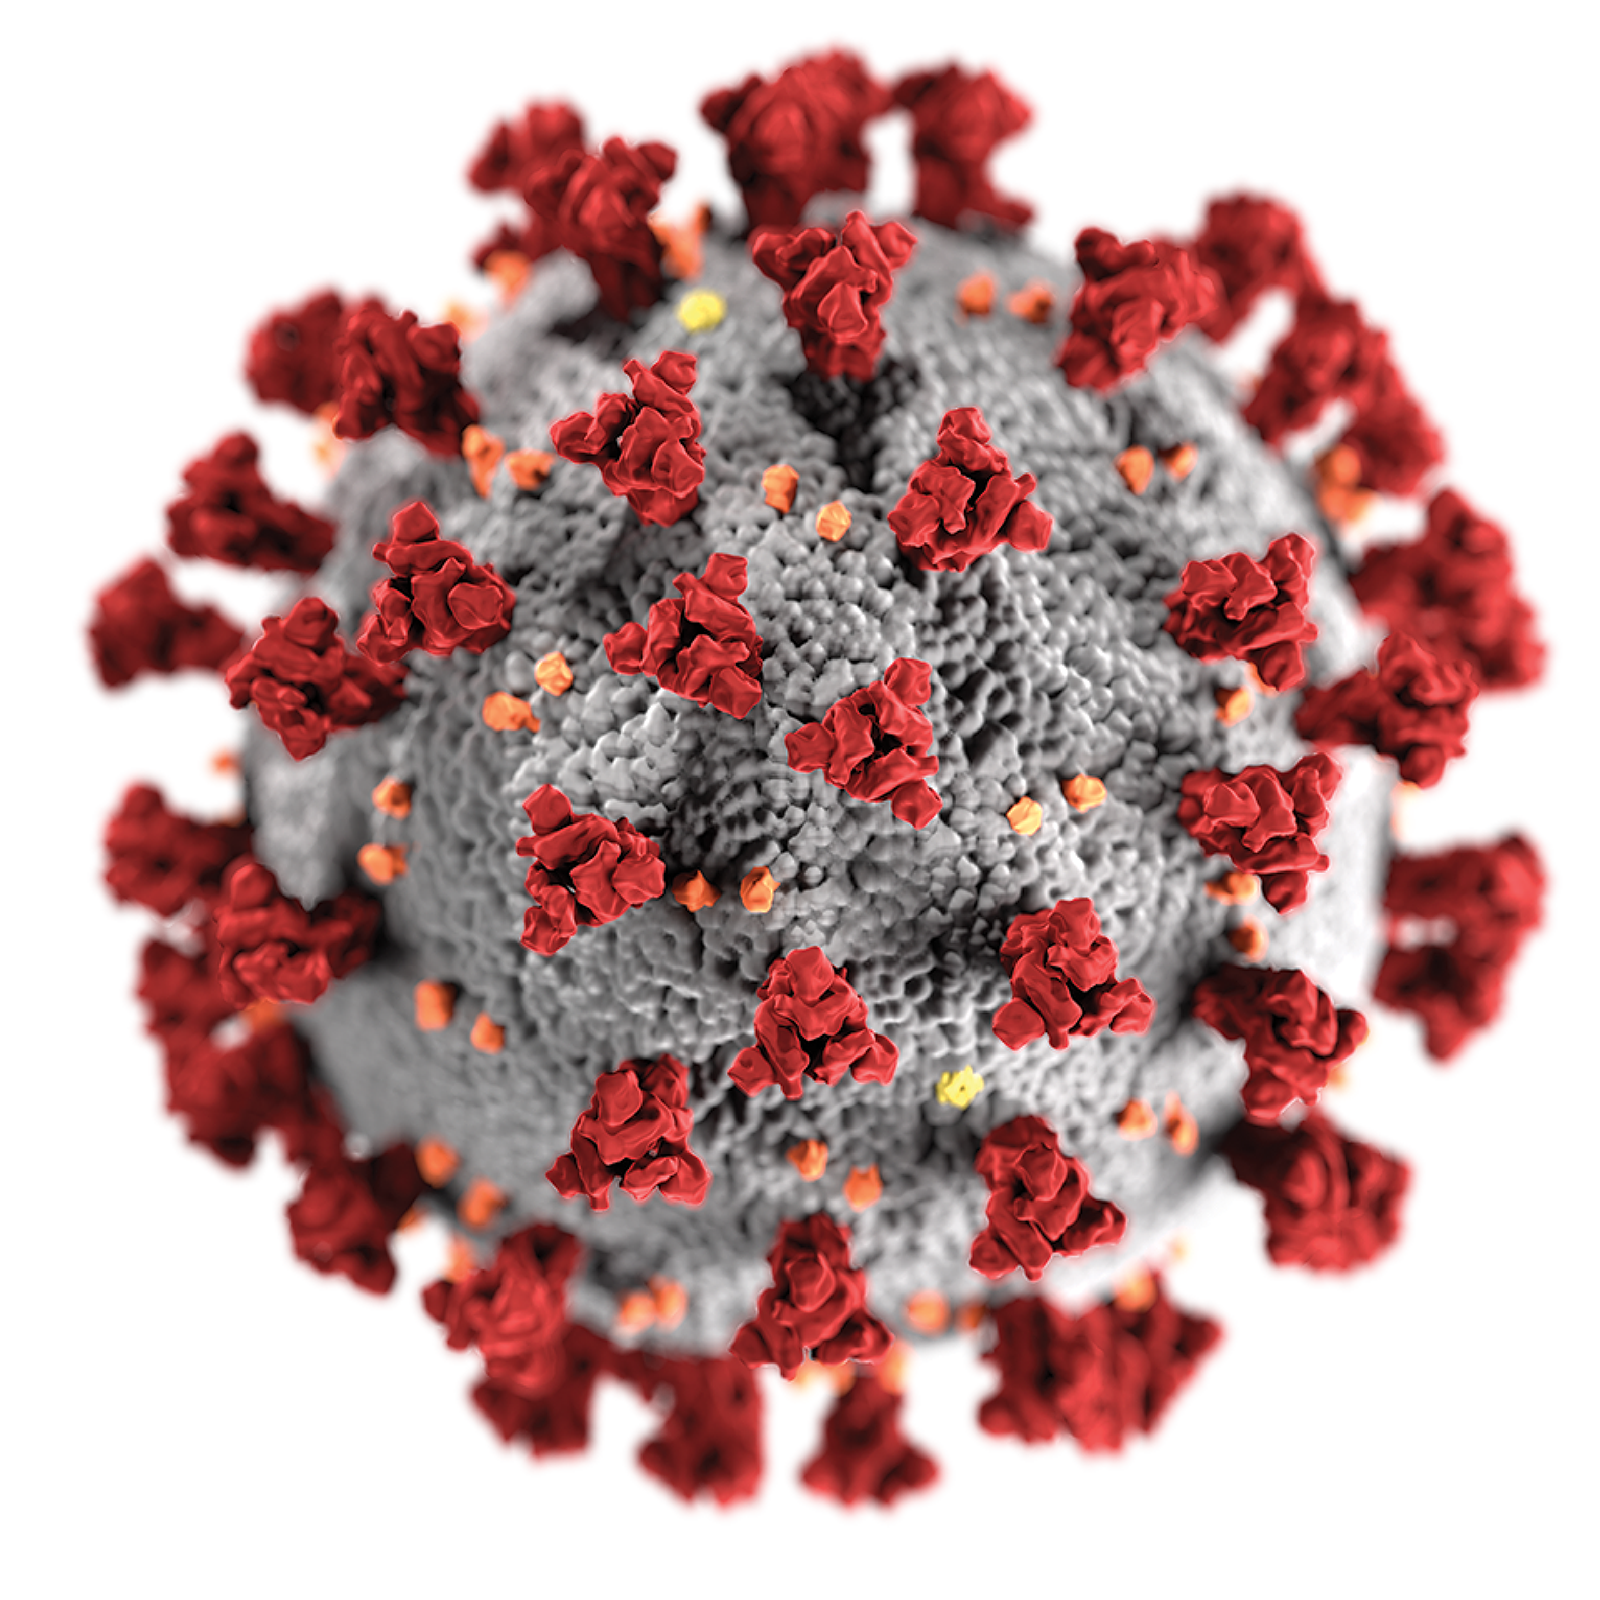
\includegraphics[width=\textwidth]{img/webinar/covid3d}
				\caption{Visualización 3D del virus COVID-19.}
			\end{figure}
		\end{column}
	\end{columns}	
\end{frame}
%-------------------------------------------------------
%-------------------------------------------------------

%-------------------------------------------------------
%-------------------------------------------------------
\begin{frame}{Muertes por Cáncer}{}
	\begin{columns}
		\begin{column}{0.48\textwidth}
			\begin{block}{}
				\textbf{3.35 millones} muertes por Cáncer en el mundo (2022) \cite{worldometrcancer2022}.
			\end{block}
			\begin{block}{}
				\textbf{9.89 millones} de muertes por Cáncer en el mundo \cite{worldometrcancer2022}.
			\end{block}
		\end{column}
		\begin{column}{0.48\textwidth}
			\begin{figure}[]
				\centering
				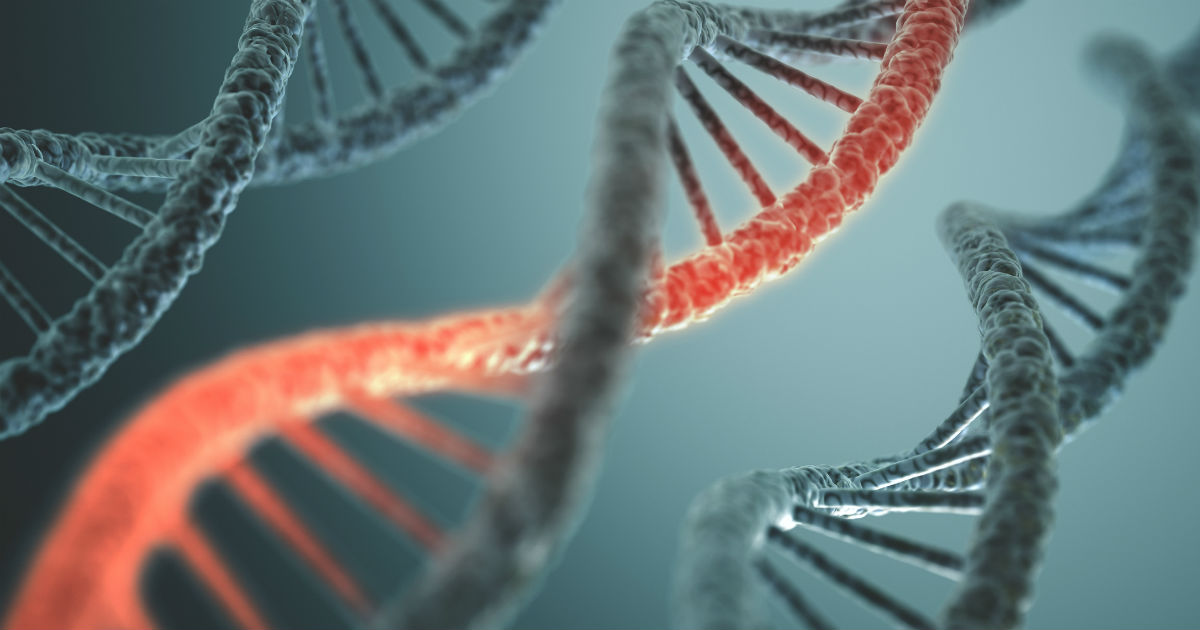
\includegraphics[width=\textwidth]{img/webinar/cancer_dna}
				\caption{Muertes por Cáncer en Perú en el 2020.}
			\end{figure}
		\end{column}
	\end{columns}	
\end{frame}
%-------------------------------------------------------
%-------------------------------------------------------

%-------------------------------------------------------
%-------------------------------------------------------
\begin{frame}{Reflexión}{}
	\begin{block}{}
		La Bioinformática representa un factor clave para el control de estas enfermedades.
	\end{block}
\end{frame}
%-------------------------------------------------------
%-------------------------------------------------------

%%%%%%%%%%%%%%%%%%%%%%%%%%%%%%%%%%%%%%%%%%%%%%%%%%%%%%%%
\subsection{Proposito de la Bioinformática}
%%%%%%%%%%%%%%%%%%%%%%%%%%%%%%%%%%%%%%%%%%%%%%%%%%%%%%%%

%-------------------------------------------------------
%-------------------------------------------------------
\begin{frame}{Proposito de la Bioinformática}{¿Porque nos enfermamos de Cáncer?}
	\begin{figure}[]
		\centering
		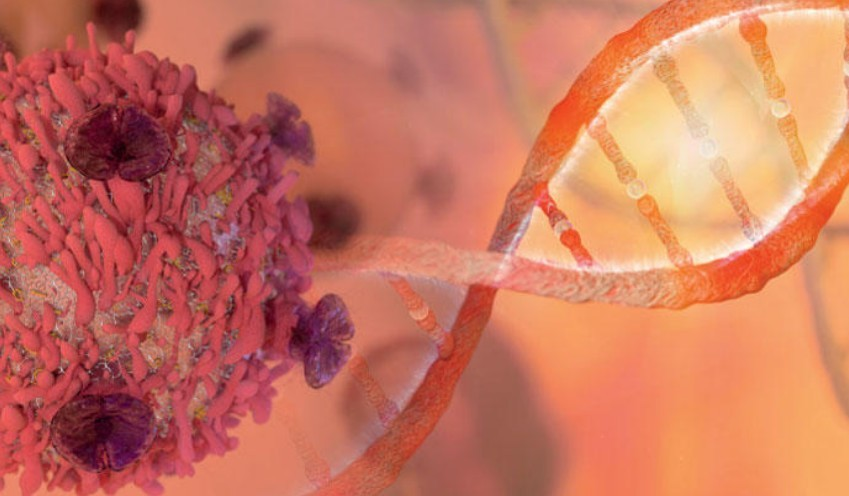
\includegraphics[width=0.9\textwidth,height=0.6\textheight]{img/introduction/mot3.jpg}
		\caption{¿Porque una persona se enferma de Cáncer?}
	\end{figure}
\end{frame}
%-------------------------------------------------------
%-------------------------------------------------------

%-------------------------------------------------------
%-------------------------------------------------------
\begin{frame}{Proposito de la Bioinformática}{Descubrimiento de nuevos medicamentos}
	\begin{figure}[]
		\centering
		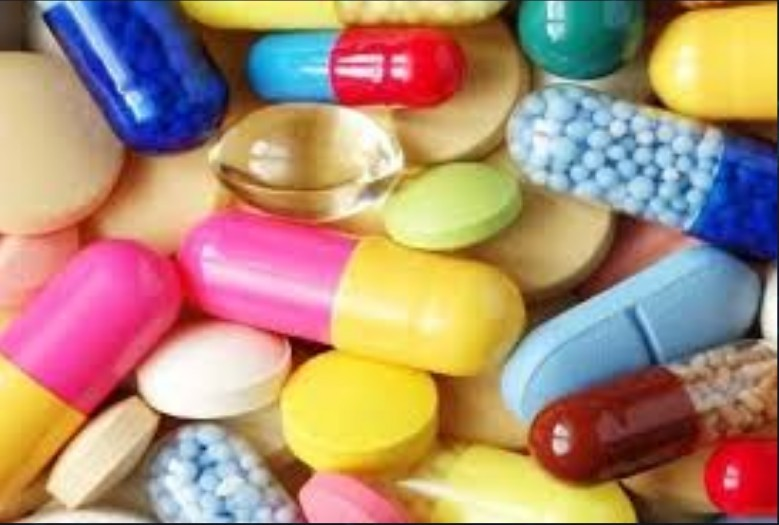
\includegraphics[width=0.9\textwidth,height=0.6\textheight]{img/introduction/mot4.jpg}
		\caption{Descubrimiento de nuevos medicamentos.}
	\end{figure}
\end{frame}
%-------------------------------------------------------
%-------------------------------------------------------

%-------------------------------------------------------
%-------------------------------------------------------
\begin{frame}{Proposito de la Bioinformática}{Medicina personalizada}
	\begin{figure}[]
		\centering
		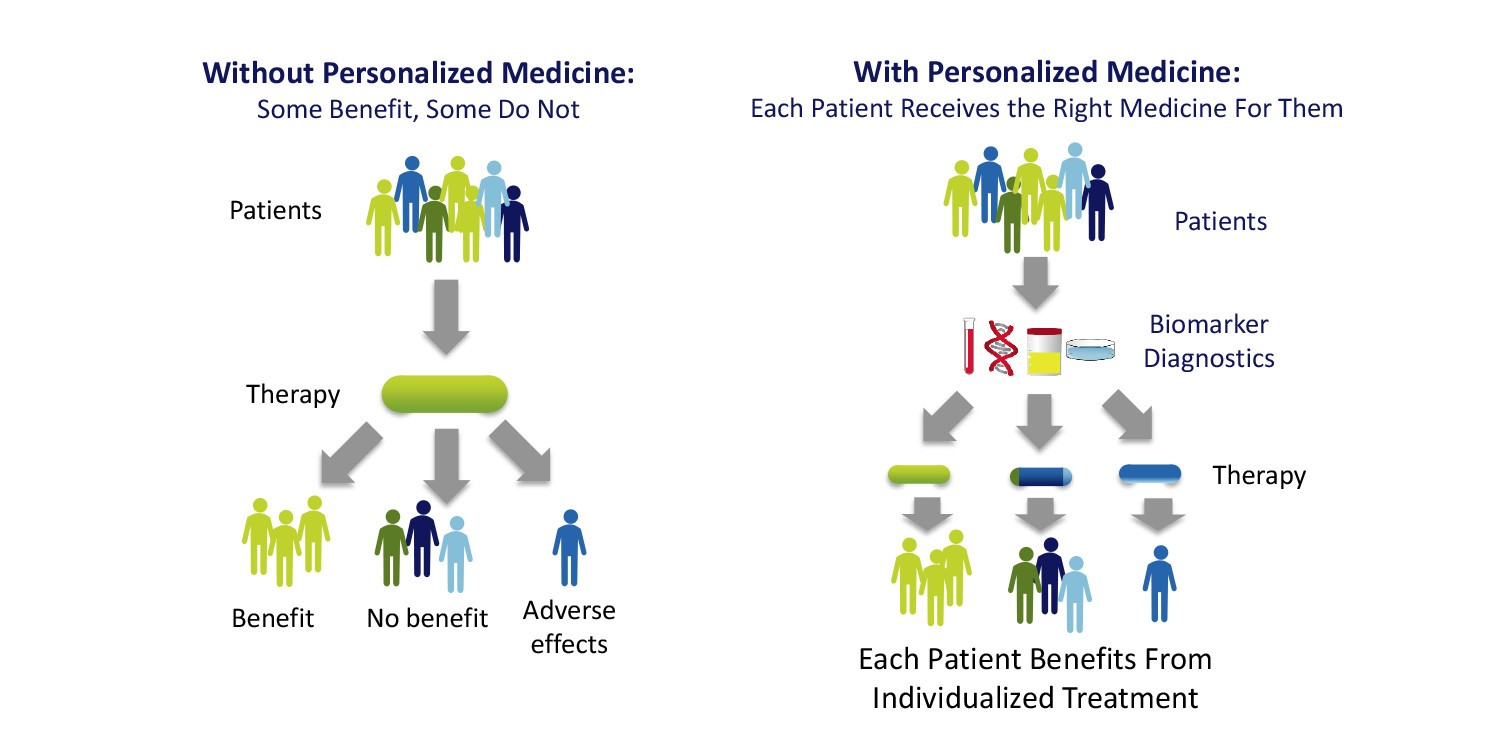
\includegraphics[width=0.9\textwidth,height=0.6\textheight]{img/introduction/mot5.jpg}
		\caption{Medicina personalizada.}
	\end{figure}
\end{frame}
%-------------------------------------------------------
%-------------------------------------------------------

%-------------------------------------------------------
%-------------------------------------------------------
\begin{frame}{Proposito de la Bioinformática}{¿Existe un gen de la bondad?}
	\begin{figure}[]
		\centering
		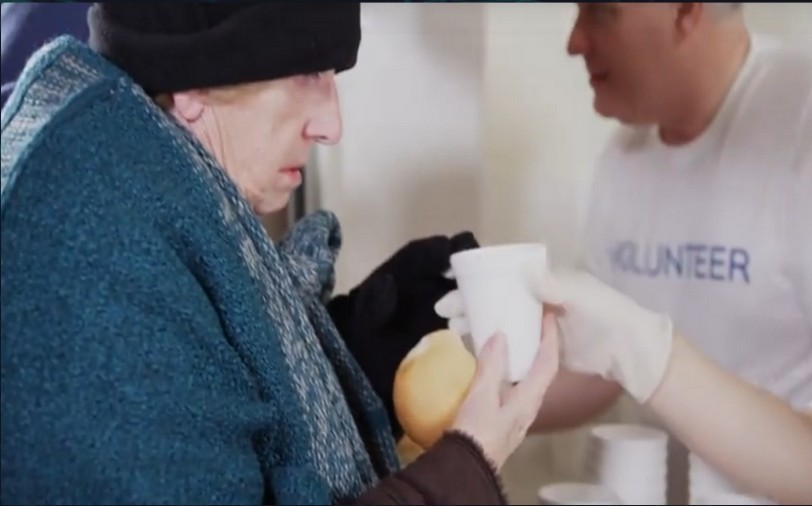
\includegraphics[width=0.9\textwidth,height=0.6\textheight]{img/introduction/mot2.jpg}
		\caption{¿Existe un gen de la bondad?}
	\end{figure}
\end{frame}
%-------------------------------------------------------
%-------------------------------------------------------

%%%%%%%%%%%%%%%%%%%%%%%%%%%%%%%%%%%%%%%%%%%%%%%%%%%%%%%%
\section{Bioinformática}
%%%%%%%%%%%%%%%%%%%%%%%%%%%%%%%%%%%%%%%%%%%%%%%%%%%%%%%%

%%%%%%%%%%%%%%%%%%%%%%%%%%%%%%%%%%%%%%%%%%%%%%%%%%%%%%%%
\subsection{Definición}
%%%%%%%%%%%%%%%%%%%%%%%%%%%%%%%%%%%%%%%%%%%%%%%%%%%%%%%%

%-------------------------------------------------------
%-------------------------------------------------------
\begin{frame}{Bioinformática}{Definición}	
	La Bioinformática involucra el uso de la tecnología de las computadoras para almacenar, recuperar, manipular y distribuir información relacionada a Biología Molecular como: \textbf{DNA, RNA, y proteínas} \cite{luscombe2001bioinformatics}.
	
\end{frame}
%-------------------------------------------------------
%-------------------------------------------------------


%-------------------------------------------------------
%-------------------------------------------------------
\begin{frame}{Bioinformática}
	\begin{figure}[]
		\centering
		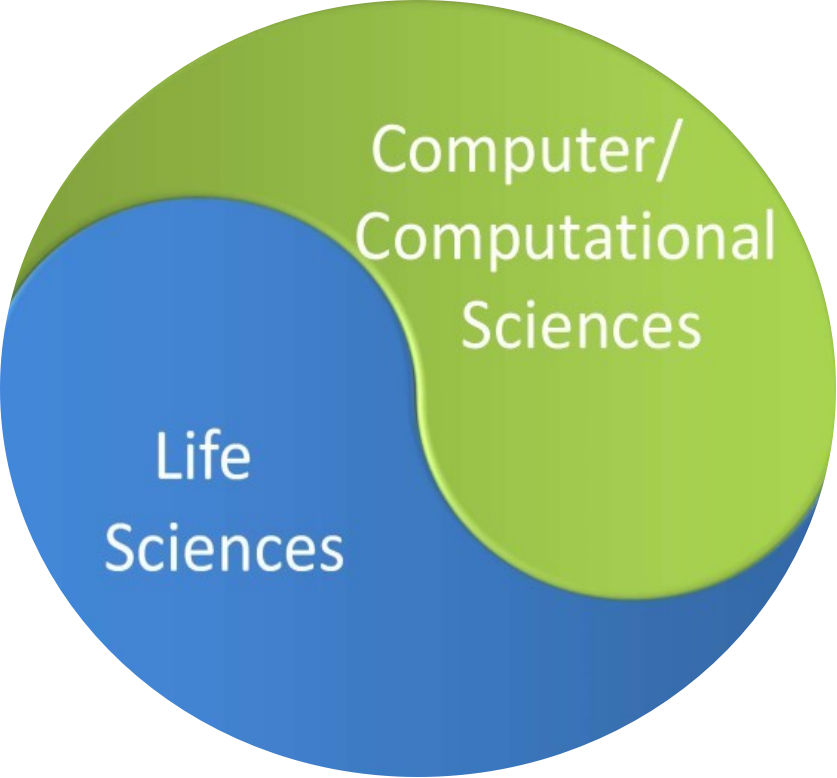
\includegraphics[width=\textwidth,height=0.7\textheight,keepaspectratio]{img/webinar/bio2.png}
		\label{img:mot2}
		%\caption{Computer simulation of protein-ligand.}
	\end{figure}
\end{frame}
%-------------------------------------------------------
%-------------------------------------------------------

%-------------------------------------------------------
%-------------------------------------------------------
\begin{frame}{Bioinformática}
	\begin{figure}[]
		\centering
		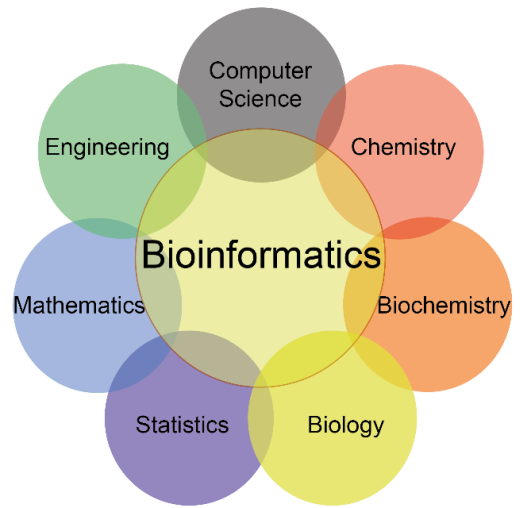
\includegraphics[width=\textwidth,height=0.7\textheight,keepaspectratio]{img/webinar/bio4}
		%\caption{Computer simulation of protein-ligand.}
	\end{figure}
\end{frame}
%-------------------------------------------------------
%-------------------------------------------------------


%-------------------------------------------------------
%-------------------------------------------------------
\begin{frame}{Bioinformática}{¿Donde está el DNA?}
	\begin{figure}[]
		\centering
		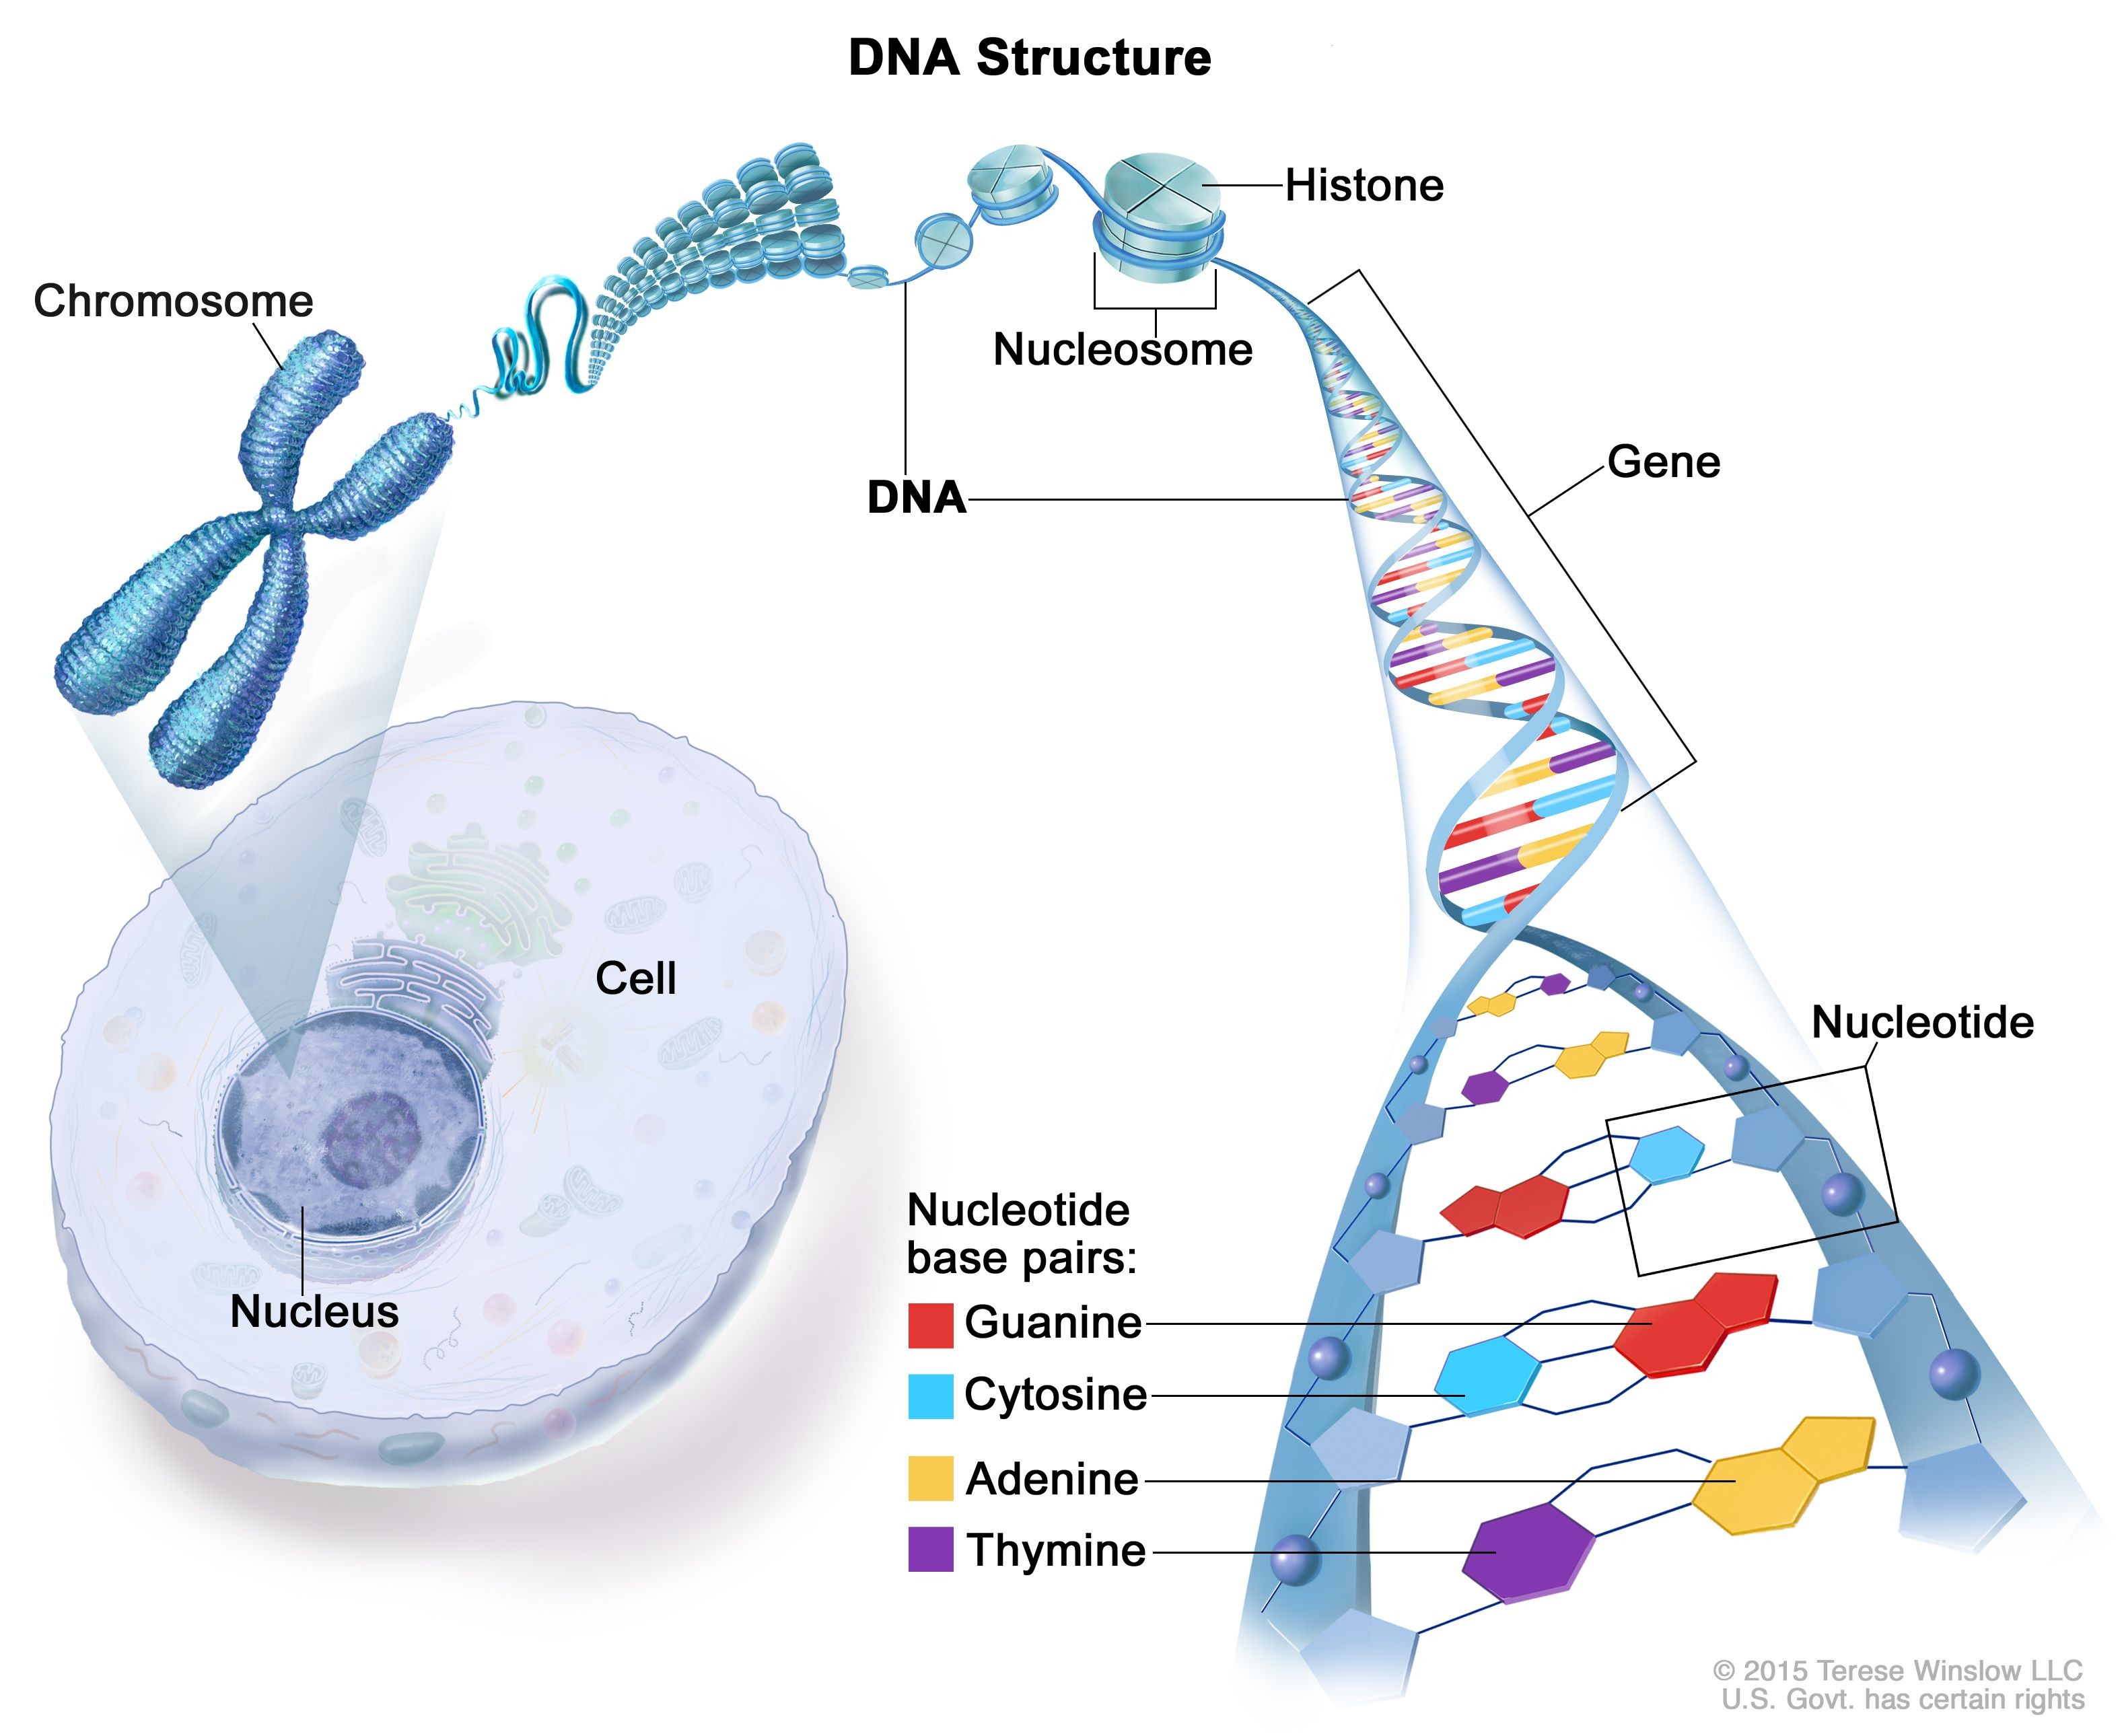
\includegraphics[width=0.7\textwidth]{img/webinar/dna}
		\caption{¿Donde está el DNA? \cite{NCIdictionary2022}.}
	\end{figure}
\end{frame}
%-------------------------------------------------------
%-------------------------------------------------------

%-------------------------------------------------------
%-------------------------------------------------------
\begin{frame}{Bioinformática}{Ejemplo de una secuencia de DNA}
	\begin{figure}[]
		\centering
		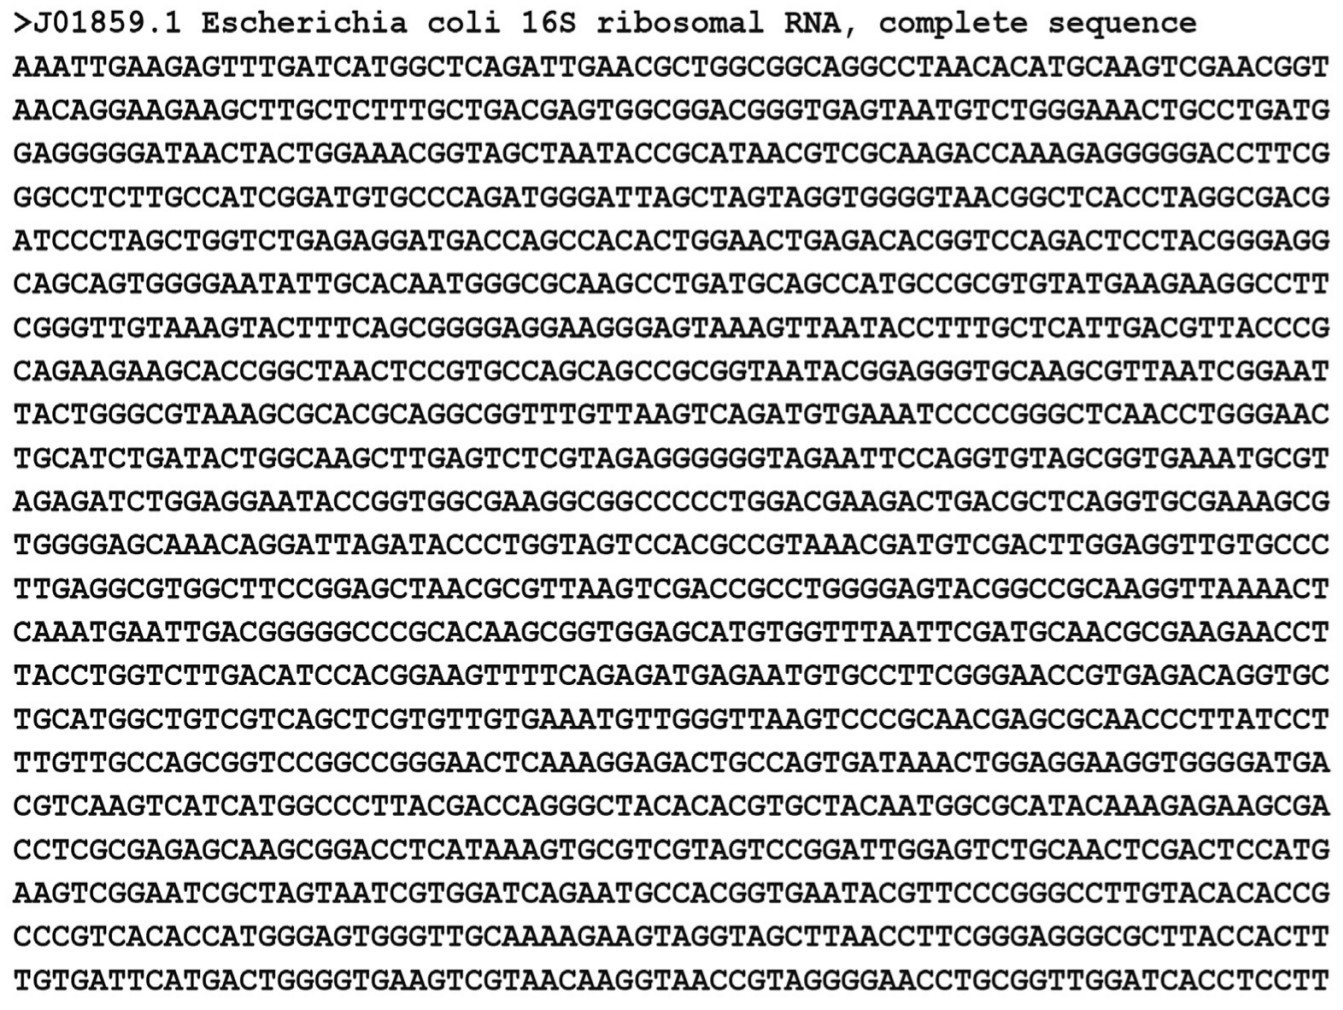
\includegraphics[width=0.9\textwidth,height=0.6\textheight]{img/webinar/dnaimg_1}
		\caption{16S ribosomal DNA of Escherichia coli with FASTA Format.}
	\end{figure}
\end{frame}
%-------------------------------------------------------
%-------------------------------------------------------

%-------------------------------------------------------
%-------------------------------------------------------
\begin{frame}{Bioinformática}{Algunos números}
	
	\begin{block}{}
		\centering
		Un genoma completo tiene \textbf{\string ~3.2 billones de bp}. \\
		\string ~6.4 billones de bases \cite{archibald2018genomics}.
	\end{block}
	
	\pause
	\begin{block}{}
		\centering
		El genoma del virus \textbf{HIV-1} tiene aproximadamente \textbf{\string ~20k bp}. \\
		El genoma del virus \textbf{COVID-19} tiene aproximadamente \textbf{\string ~32k bp} \cite{randhawa2020machine}.
	\end{block}
	
	\pause
	\begin{block}{}
		\centering
		Existe aproximadamente \textbf{19000} a \textbf{25000} genes \cite{archibald2018genomics}.
	\end{block}
	
\end{frame}
%-------------------------------------------------------
%-------------------------------------------------------

%-------------------------------------------------------
%-------------------------------------------------------
\begin{frame}{Bioinformática}{Transcripción y Traducción}
	\begin{figure}[]
		\centering
		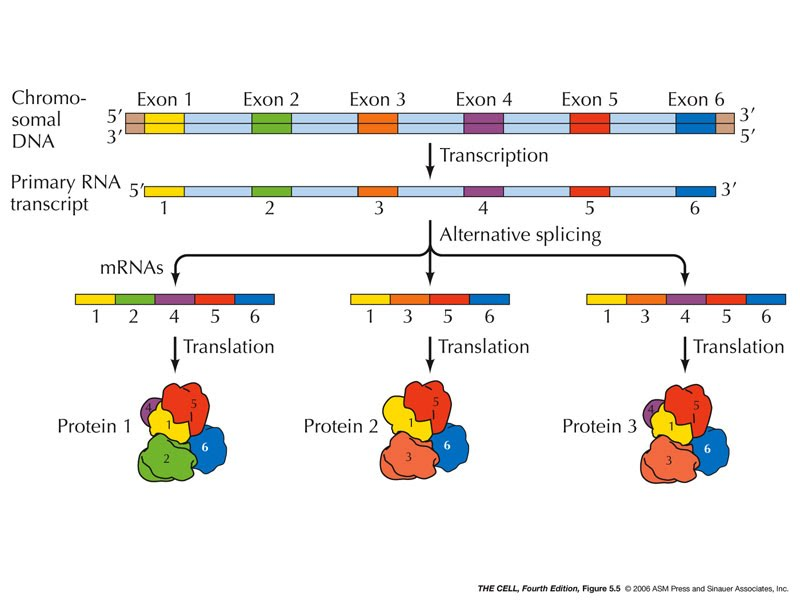
\includegraphics[width=0.9\textwidth]{img/numbers/alt.jpg}
		\caption{Alternative splicing \cite{genbio2020}.}
	\end{figure}
\end{frame}
%-------------------------------------------------------
%-------------------------------------------------------



%%%%%%%%%%%%%%%%%%%%%%%%%%%%%%%%%%%%%%%%%%%%%%%%%%%%%%%%%%%%%%%%%%%%%%%%%%%%%%%%%%%%%%%
%%%%%%%%%%%%%%%%%%%%%%%%%%%%%%%%%%%%%%%%%%%%%%%%%%%%%%%%%%%%%%%%%%%%%%%%%%%%%%%%%%%%%%%
\section{Aplicaciones}
%%%%%%%%%%%%%%%%%%%%%%%%%%%%%%%%%%%%%%%%%%%%%%%%%%%%%%%%%%%%%%%%%%%%%%%%%%%%%%%%%%%%%%%
%%%%%%%%%%%%%%%%%%%%%%%%%%%%%%%%%%%%%%%%%%%%%%%%%%%%%%%%%%%%%%%%%%%%%%%%%%%%%%%%%%%%%%%

%%%%%%%%%%%%%%%%%%%%%%%%%%%%%%%%%%%%%%%%%%%%%%%%%%%%%%%%%%%%%%%%%%%%%%%%%%%%%%%%%%%%%%%
%%%%%%%%%%%%%%%%%%%%%%%%%%%%%%%%%%%%%%%%%%%%%%%%%%%%%%%%%%%%%%%%%%%%%%%%%%%%%%%%%%%%%%%
\subsection{Alineamiento y árboles filogenéticos}
%%%%%%%%%%%%%%%%%%%%%%%%%%%%%%%%%%%%%%%%%%%%%%%%%%%%%%%%%%%%%%%%%%%%%%%%%%%%%%%%%%%%%%%
%%%%%%%%%%%%%%%%%%%%%%%%%%%%%%%%%%%%%%%%%%%%%%%%%%%%%%%%%%%%%%%%%%%%%%%%%%%%%%%%%%%%%%%

%-------------------------------------------------------
%-------------------------------------------------------
\begin{frame}{Aplicaciones de la Bioinformática}{Origenes del COVID-19}
	\begin{figure}[]
		\centering
		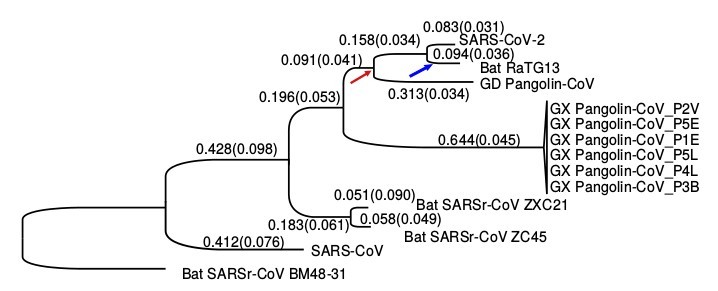
\includegraphics[width=\textwidth,height=0.7\textheight,keepaspectratio]{img/alignment/phylocovid.jpg}
		\caption{Árbol filogenético del COVID-19 y otros coronavirus \cite{tang2020origin}.}
	\end{figure}
\end{frame}
%-------------------------------------------------------
%-------------------------------------------------------

%-------------------------------------------------------
%-------------------------------------------------------
\begin{frame}{Aplicaciones de la Bioinformática}{Métodos alternátivos de alineamiento}
	\begin{block}{}
		An Analysis of k-Mer Frequency Features with Machine Learning Models for Viral Subtyping of Polyomavirus and HIV-1 Genomes \cite{arceda2020analysis}.
	\end{block}

	\begin{block}{}
		An analysis of k-mer frequency features with SVM and CNN for viral subtyping classification \cite{machaca2020analysis}.
	\end{block}
\end{frame}
%-------------------------------------------------------
%-------------------------------------------------------



%%%%%%%%%%%%%%%%%%%%%%%%%%%%%%%%%%%%%%%%%%%%%%%%%%%%%%%%%%%%%%%%%%%%%%%%%%%%%%%%%%%%%%%
%%%%%%%%%%%%%%%%%%%%%%%%%%%%%%%%%%%%%%%%%%%%%%%%%%%%%%%%%%%%%%%%%%%%%%%%%%%%%%%%%%%%%%%
\subsection{Predicción de estructuras de proteínas}
%%%%%%%%%%%%%%%%%%%%%%%%%%%%%%%%%%%%%%%%%%%%%%%%%%%%%%%%%%%%%%%%%%%%%%%%%%%%%%%%%%%%%%%
%%%%%%%%%%%%%%%%%%%%%%%%%%%%%%%%%%%%%%%%%%%%%%%%%%%%%%%%%%%%%%%%%%%%%%%%%%%%%%%%%%%%%%%

%-------------------------------------------------------
%-------------------------------------------------------
\begin{frame}{Aplicaciones de la Bioinformática}{Predicción de estructuras de proteínas}
	\begin{figure}[]
		\centering
		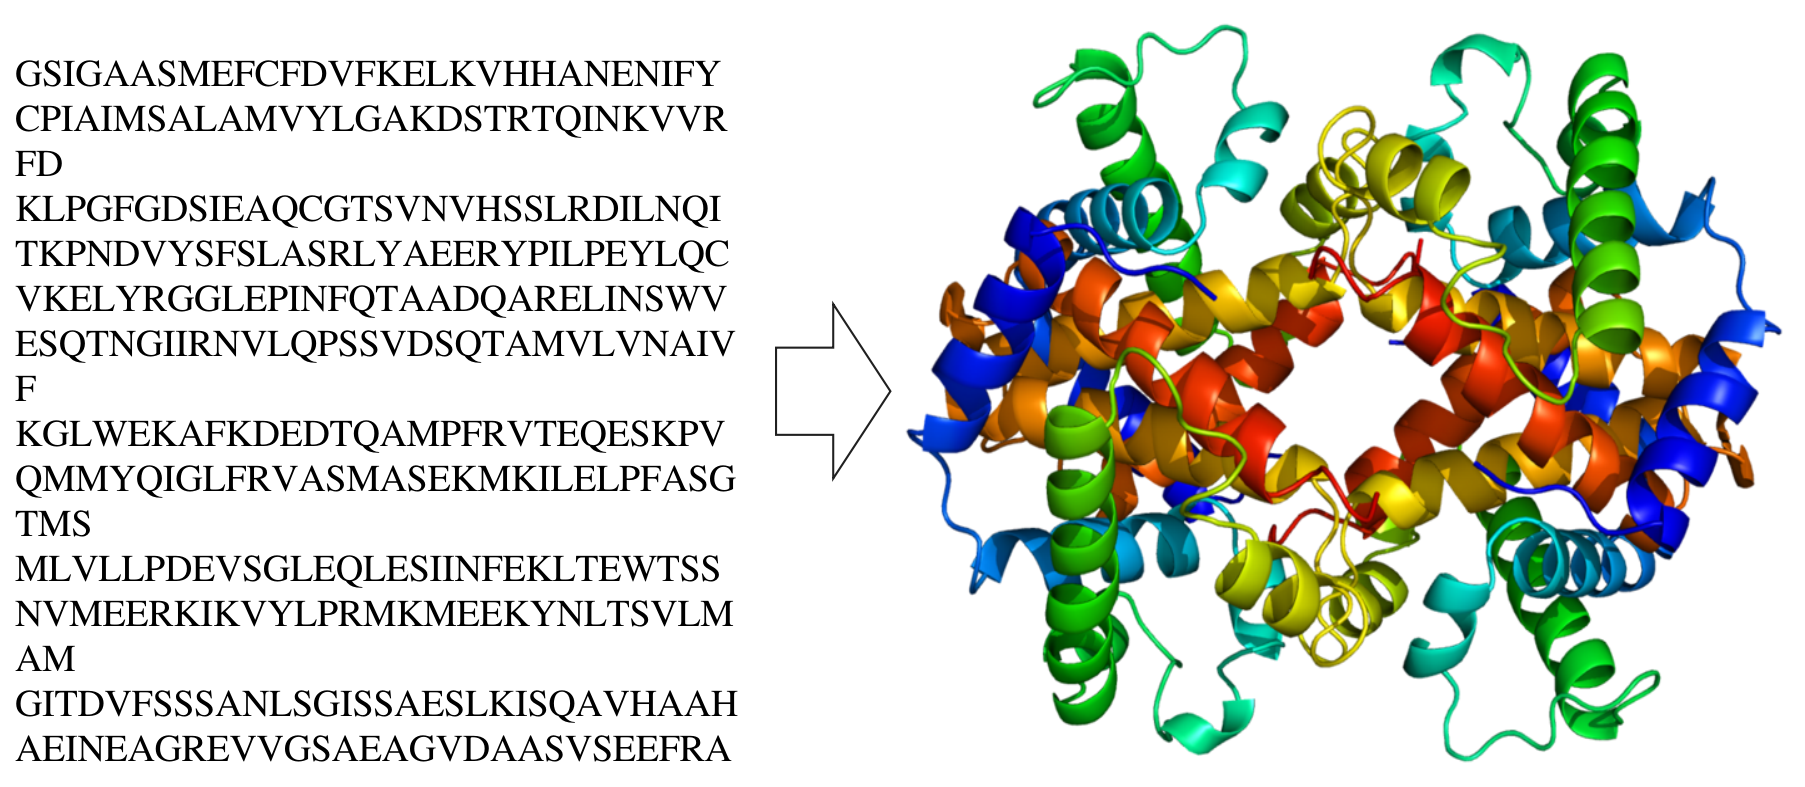
\includegraphics[width=\textwidth]{img/webinar/psp2}
		\caption{Simulación 3D de la estructura terciaría de una proteína.}
	\end{figure}
\end{frame}
%-------------------------------------------------------
%-------------------------------------------------------

%-------------------------------------------------------
%-------------------------------------------------------
\begin{frame}{Protein structure prediction}{Método propuesto por AlphaFold}
	\begin{figure}[]
		\centering
		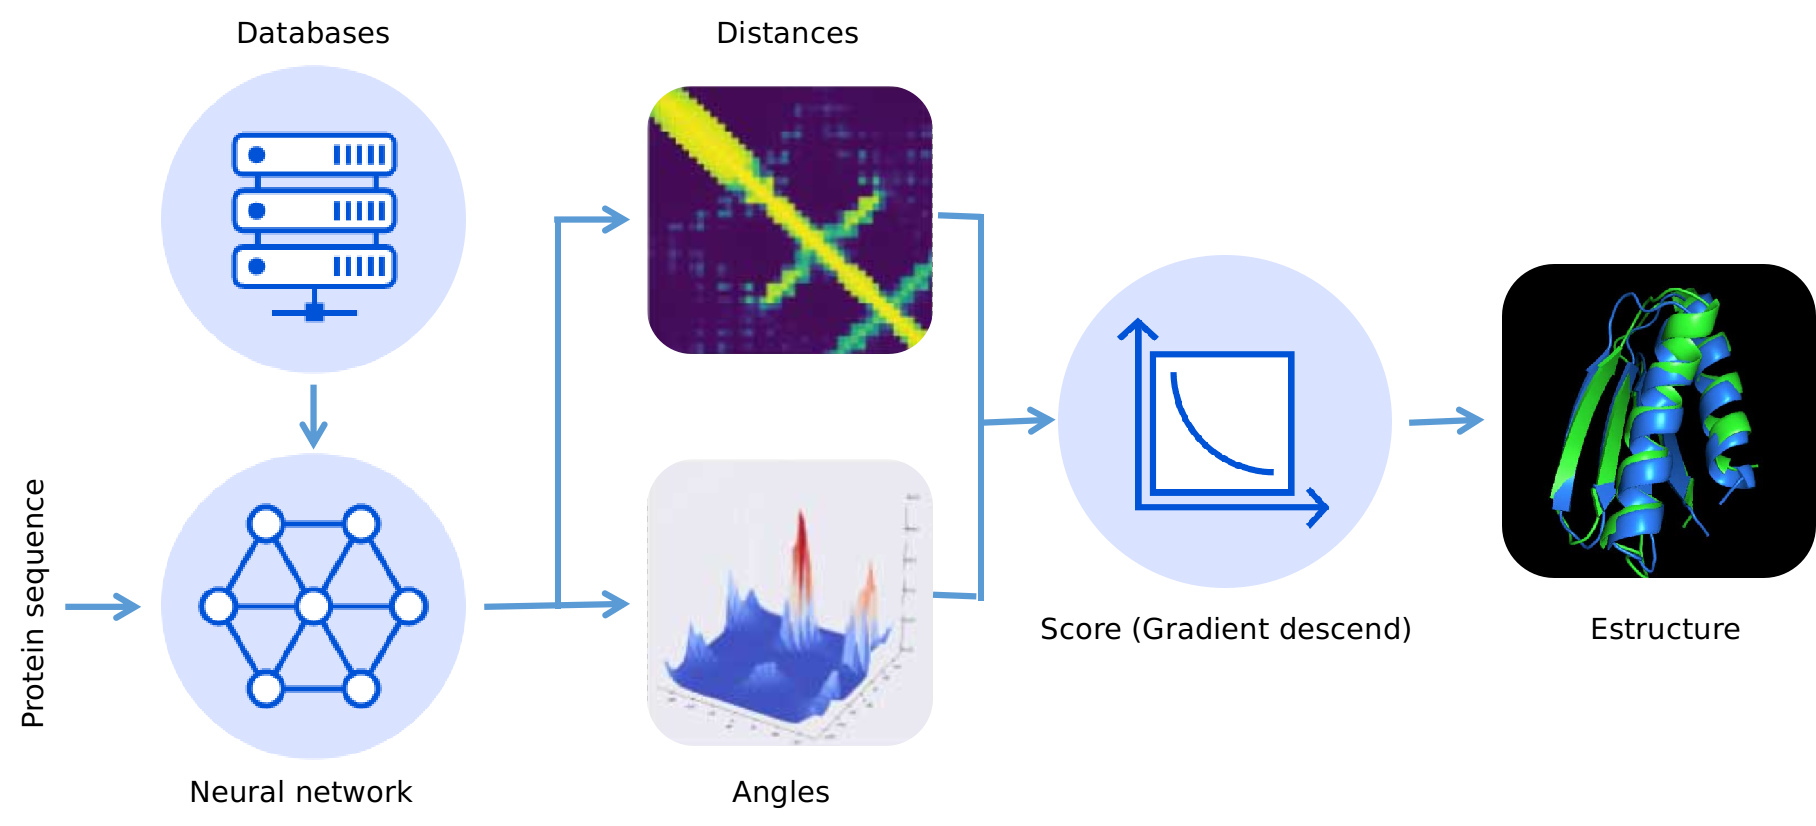
\includegraphics[width=\textwidth,keepaspectratio]{img/webinar/protein_prediction}
		\caption{Predicción de estructuras de proteínas con AlphaFold \cite{alphafold2020}.}
	\end{figure}
\end{frame}
%-------------------------------------------------------
%-------------------------------------------------------

%-------------------------------------------------------
%-------------------------------------------------------
\begin{frame}{Protein structure prediction}{ArgosMol}
	\begin{figure}[]
		\centering
		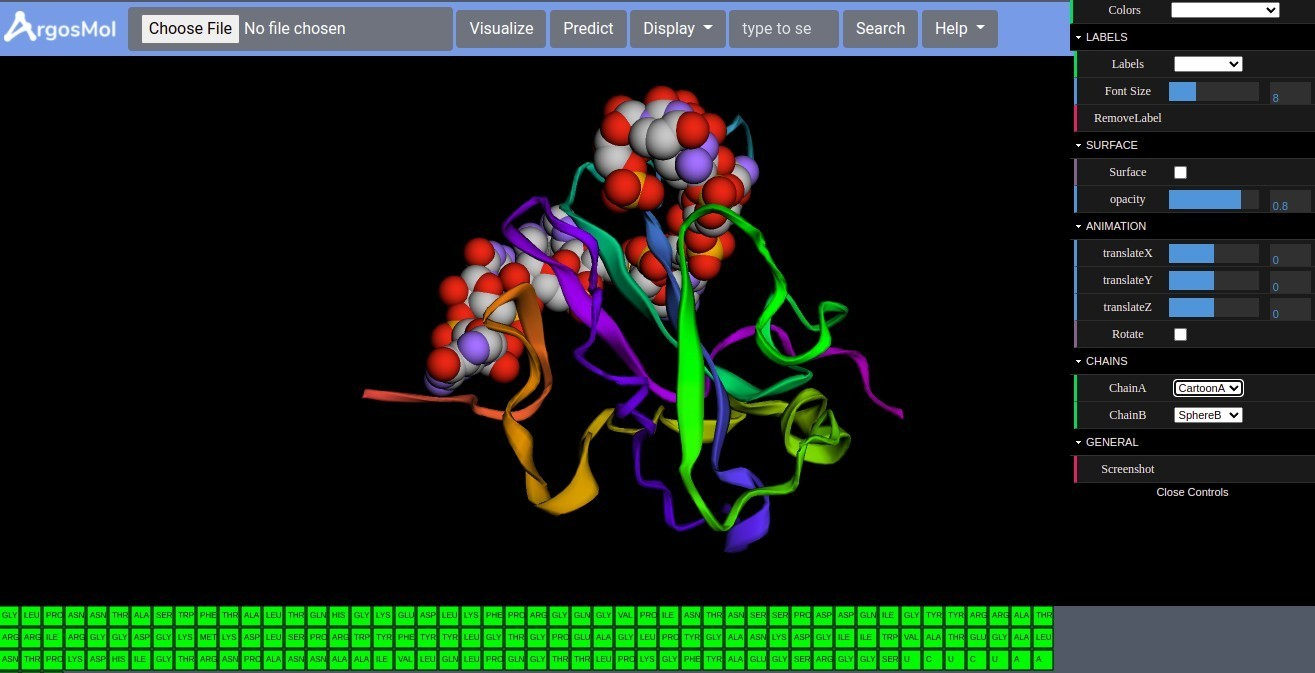
\includegraphics[width=\textwidth,keepaspectratio]{img/webinar/argosmol}
		\caption{ArgosMol: \chref{http://143.244.188.93:8080/}{http://143.244.188.93:8080}  \cite{condori2022argosmol}.}
	\end{figure}
\end{frame}
%-------------------------------------------------------
%-------------------------------------------------------

%%%%%%%%%%%%%%%%%%%%%%%%%%%%%%%%%%%%%%%%%%%%%%%%%%%%%%%%%%%%%%%%%%%%%%%%%%%%%%%%%%%%%%%
%%%%%%%%%%%%%%%%%%%%%%%%%%%%%%%%%%%%%%%%%%%%%%%%%%%%%%%%%%%%%%%%%%%%%%%%%%%%%%%%%%%%%%%
\subsection{Descubrimiento de nuevos medicamentos}
%%%%%%%%%%%%%%%%%%%%%%%%%%%%%%%%%%%%%%%%%%%%%%%%%%%%%%%%%%%%%%%%%%%%%%%%%%%%%%%%%%%%%%%
%%%%%%%%%%%%%%%%%%%%%%%%%%%%%%%%%%%%%%%%%%%%%%%%%%%%%%%%%%%%%%%%%%%%%%%%%%%%%%%%%%%%%%%

%-------------------------------------------------------
%-------------------------------------------------------
\begin{frame}{Aplicaciones de la Bioinformática}{De un millon a uno}
	\begin{figure}[]
		\centering
		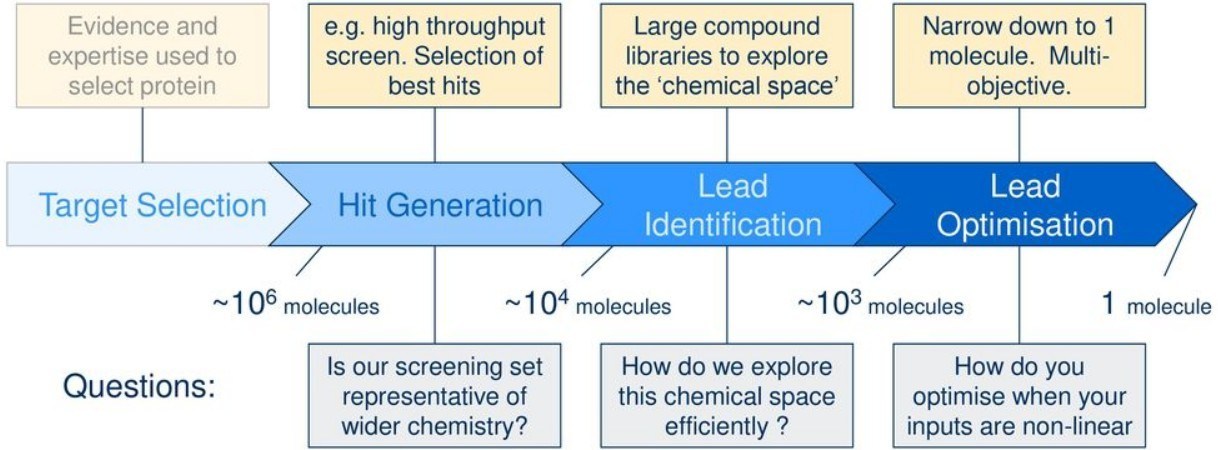
\includegraphics[width=\textwidth,keepaspectratio]{img/webinar/drug2}
		\caption{Proceso del descubrimiento de medicamentos \cite{chanin2020}.}
	\end{figure}
\end{frame}
%-------------------------------------------------------
%-------------------------------------------------------

%-------------------------------------------------------
%-------------------------------------------------------
\begin{frame}{Aplicaciones de la Bioinformática}{Descubrimiento de nuevos medicamentos}
	\begin{figure}[]
		\centering
		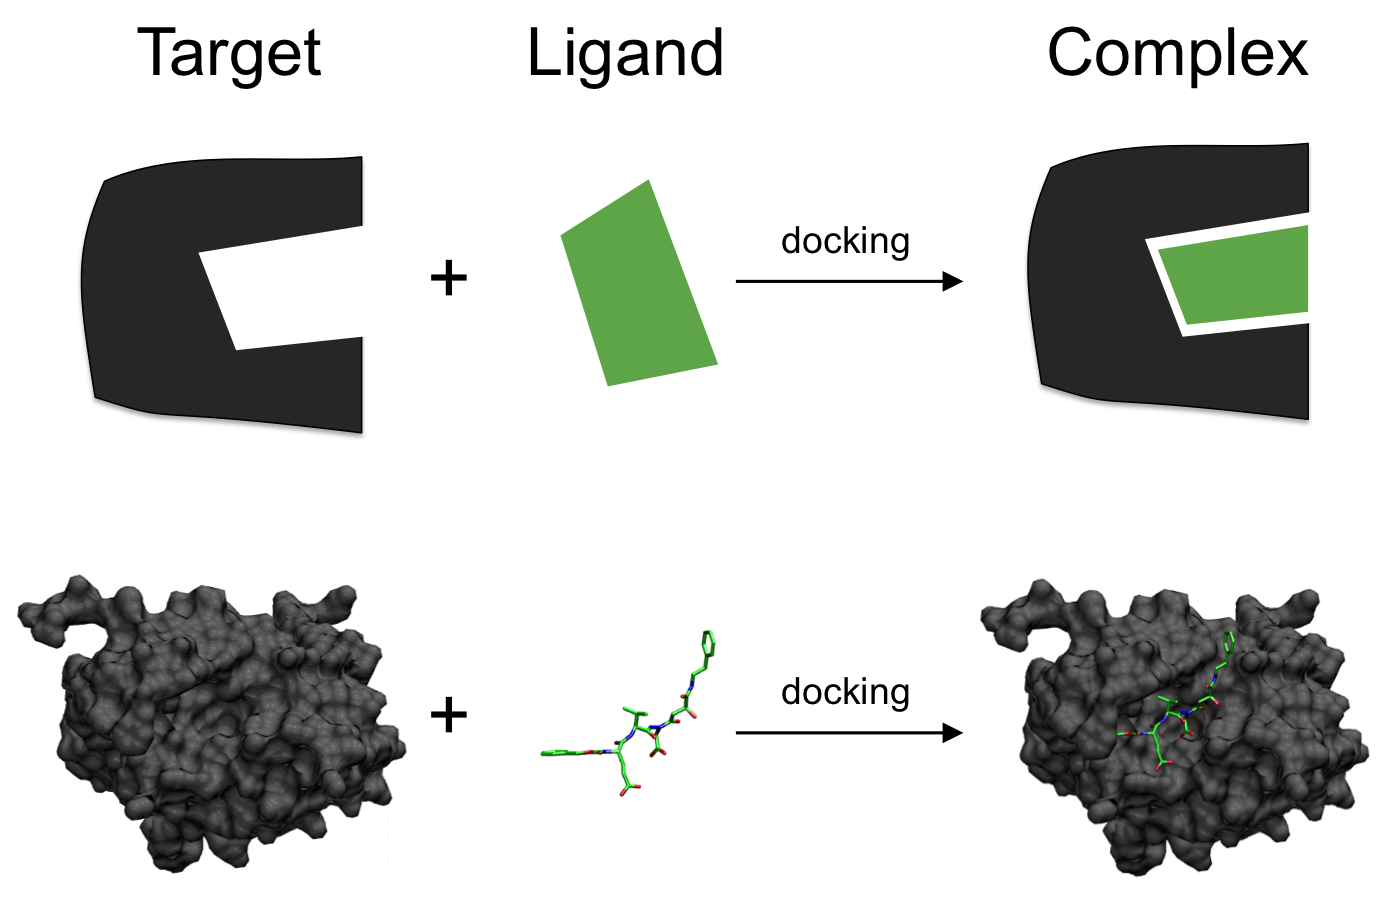
\includegraphics[width=0.9\textwidth]{img/webinar/docking}		
	\end{figure}
\end{frame}
%-------------------------------------------------------
%-------------------------------------------------------

%-------------------------------------------------------
%-------------------------------------------------------
\begin{frame}{Aplicaciones de la Bioinformática}{Descubrimiento de nuevos medicamentos}
	\begin{figure}[]
		\centering
		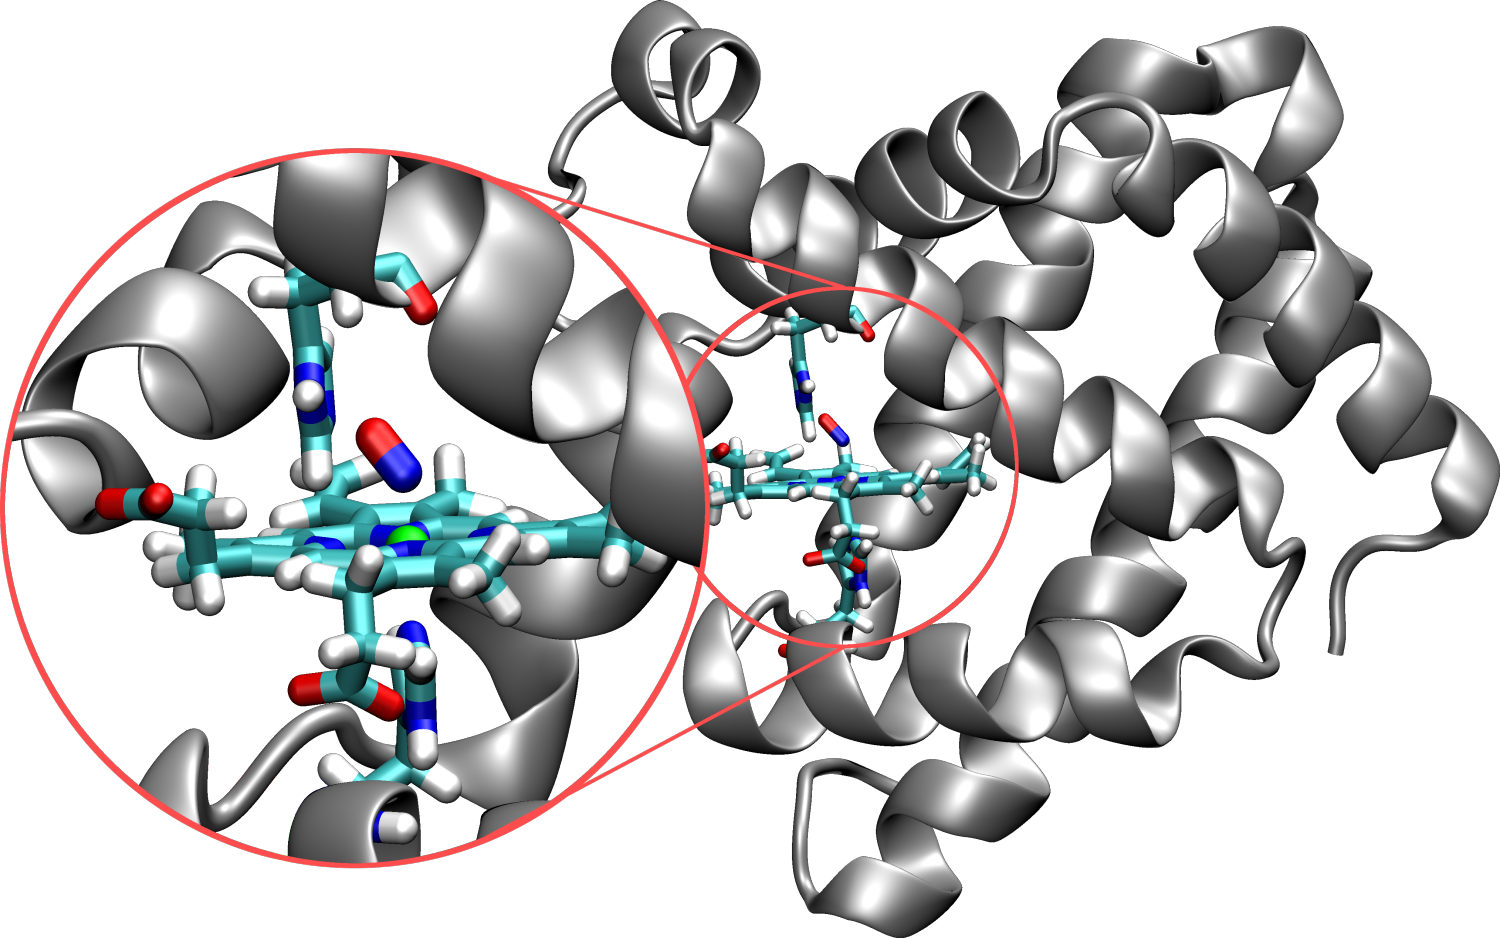
\includegraphics[width=0.8\textwidth]{img/webinar/protein2}
		\caption{Enlace entre una molécula y una proteína.}
	\end{figure}
\end{frame}
%-------------------------------------------------------
%-------------------------------------------------------


%%%%%%%%%%%%%%%%%%%%%%%%%%%%%%%%%%%%%%%%%%%%%%%%%%%%%%%%%%%%%%%%%%%%%%%%%%%%%%%%%%%%%%%
%%%%%%%%%%%%%%%%%%%%%%%%%%%%%%%%%%%%%%%%%%%%%%%%%%%%%%%%%%%%%%%%%%%%%%%%%%%%%%%%%%%%%%%
\subsection{Inmunoterapia del Cáncer}
%%%%%%%%%%%%%%%%%%%%%%%%%%%%%%%%%%%%%%%%%%%%%%%%%%%%%%%%%%%%%%%%%%%%%%%%%%%%%%%%%%%%%%%
%%%%%%%%%%%%%%%%%%%%%%%%%%%%%%%%%%%%%%%%%%%%%%%%%%%%%%%%%%%%%%%%%%%%%%%%%%%%%%%%%%%%%%%

%-------------------------------------------------------
%-------------------------------------------------------
\begin{frame}{Aplicaciones de la Bioinformática}{Inmunoterapia del Cáncer}		
	\textbf{Inmunoterapia del cancer} es un tipo de tratamiento contra el cáncer que estimula las defensas naturales del cuerpo para combatir el cáncer \cite{inmunoterapy2022}.
	
	\begin{figure}
		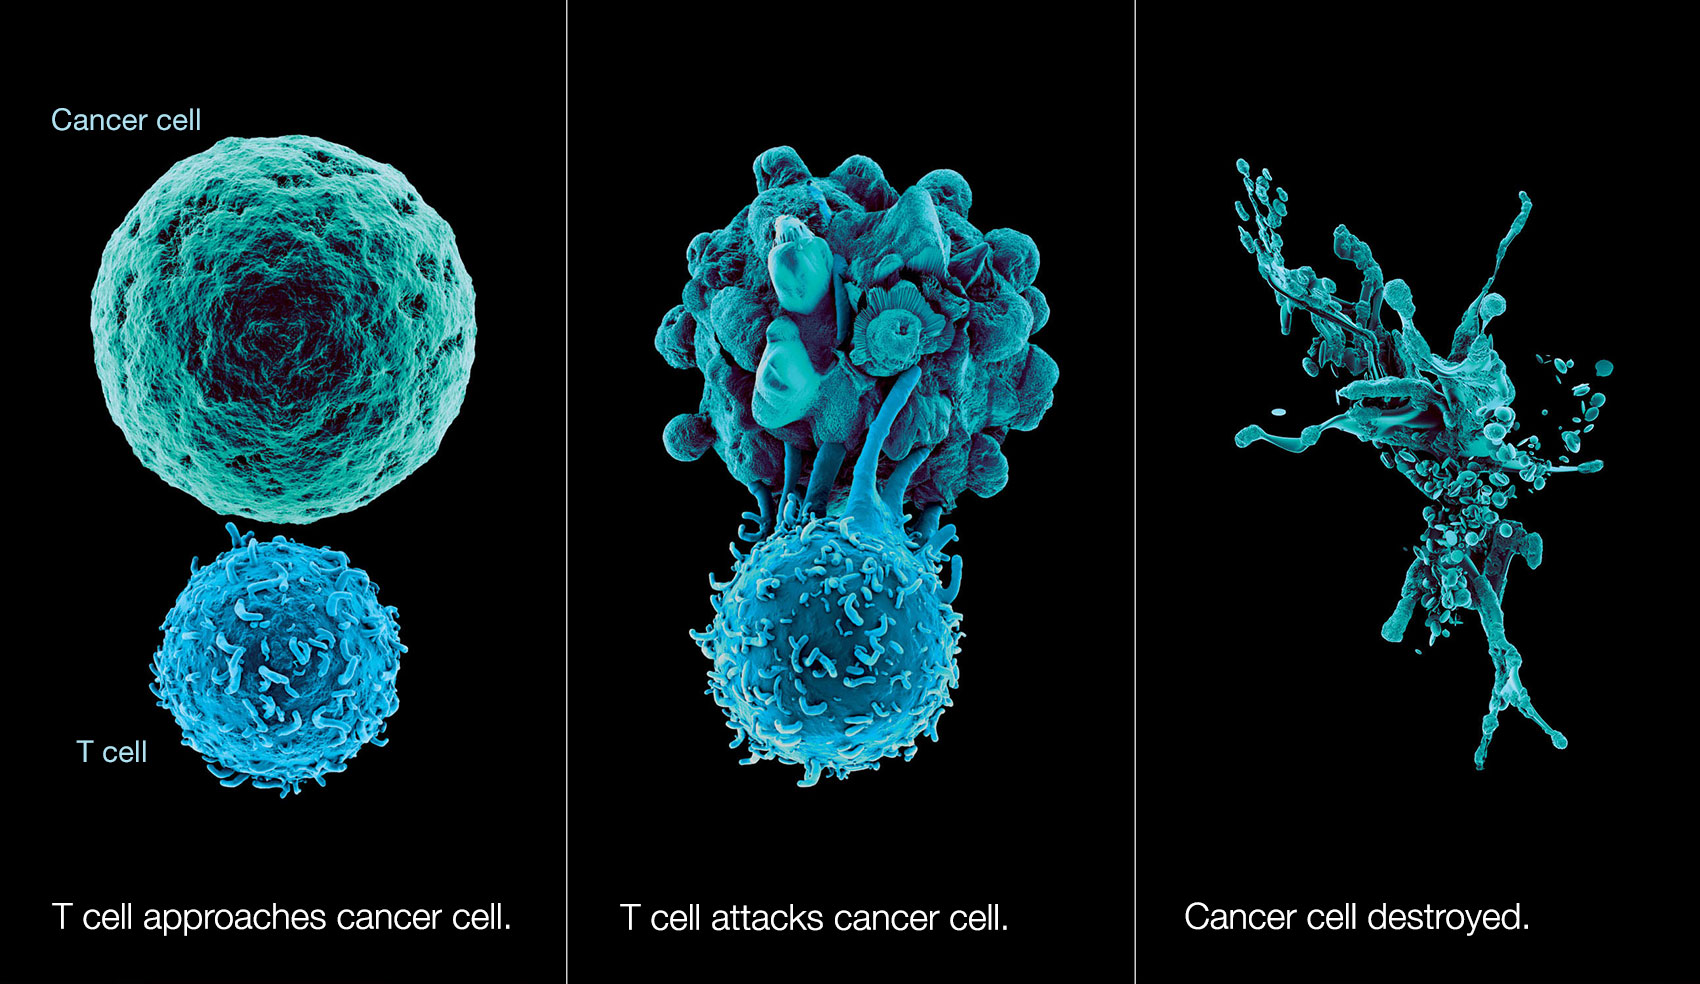
\includegraphics[width=0.7\textwidth]{img/webinar/tcell}
		\caption{Ejemplo de como una célula T, destruye células del cancer.}
	\end{figure}		
\end{frame}
%-------------------------------------------------------
%-------------------------------------------------------

%-------------------------------------------------------
%-------------------------------------------------------
\begin{frame}{Aplicaciones de la Bioinformática}{Neo antígenos}		
	\textbf{Antígeno} es cualquier sustancia que provoca que el sistema inmunitario produzca anticuerpos contra sí mismo \cite{antigen2022}.
	
	\begin{figure}
		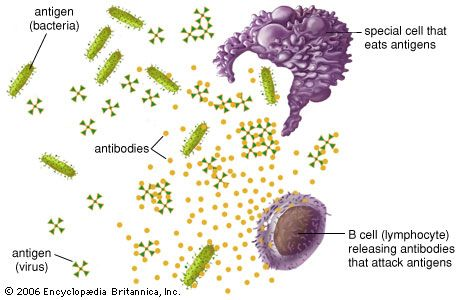
\includegraphics[width=0.6\textwidth]{img/webinar/antigen}
		\caption{Ejemplos de antígenos y como son destruídos por el sistema inmune. Fuente: \chref{https://www.britannica.com/science/antigen}{enlace}.}
	\end{figure}		
\end{frame}
%-------------------------------------------------------
%-------------------------------------------------------

%-------------------------------------------------------
%-------------------------------------------------------
\begin{frame}{Aplicaciones de la Bioinformática}{Proceso}		
	\textbf{Neo antígeno} es una proteína que se produce cuando aparecen ciertas mutaciones en el ADN de un tumor \cite{neoantigen2022}.
	
	\begin{figure}
		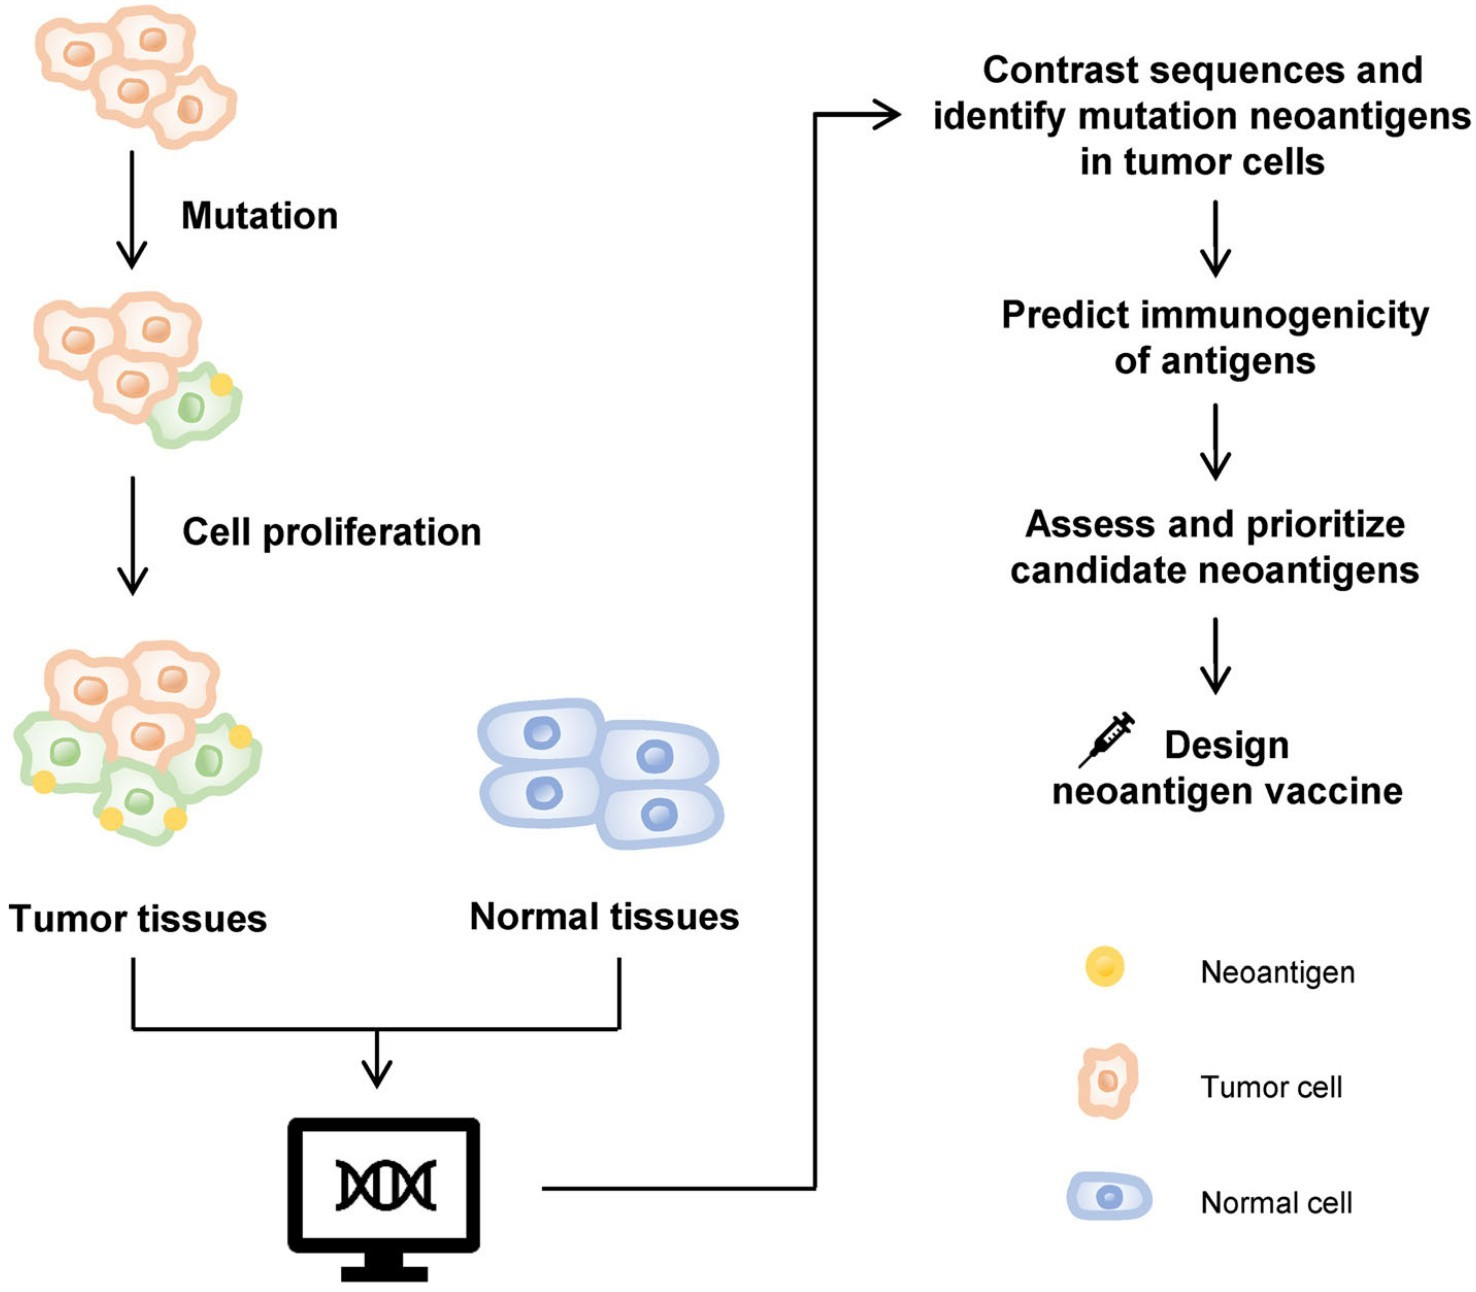
\includegraphics[width=0.5\textwidth]{img/webinar/process}
		\caption{Proceso para la generación de vacunas personalizadas contra el cáncer. Fuente: \cite{peng2019neoantigen}.}
	\end{figure}		
\end{frame}
%-------------------------------------------------------
%-------------------------------------------------------












%-------------------------------------------------------
%-------------------------------------------------------
\begin{frame}{Aplicaciones de la Bioinformática}{}
	\begin{block}{}
		Continuara...
	\end{block}
\end{frame}
%-------------------------------------------------------
%-------------------------------------------------------









%-------------------------------------------------------
%-------------------------------------------------------
\begin{frame}[allowframebreaks]
	\frametitle{References}
	%\bibliographystyle{amsalpha}
	\bibliographystyle{IEEEtran}
	\bibliography{bibliography}
\end{frame}
%-------------------------------------------------------
%-------------------------------------------------------



%-------------------------------------------------------
%-------------------------------------------------------
\if\mycmd1 % MY THEME
\1{
	{\1
		\begin{frame}[plain,noframenumbering]
			%\finalpage{Thank you}
			\begin{figure}[]
				\centering
				
\includegraphics[width=\textwidth,height=0.7\textheight,keepaspectratio]{img/question.png}
				%\label{img:mot2}
				%\caption{Image example in 2 gray levels.}
			\end{figure}
	\end{frame}}
	\else % CS THEME
	\begin{frame}{¿Preguntas?}
		\begin{figure}[]
			\centering
			
\includegraphics[width=\textwidth,height=0.7\textheight,keepaspectratio]{img/question.png}
			%\label{img:mot2}
			%\caption{Image example in 2 gray levels.}
		\end{figure}
		
	\end{frame}
	\fi
	%-------------------------------------------------------
	%-------------------------------------------------------
	

\end{document}